\documentclass[a4paper, 10pt, twocolumn]{article}
\usepackage{cellspace, graphicx, makecell}
\usepackage{graphicx} % Required for inserting images
\usepackage[utf8x]{inputenc}
\usepackage[english,russian]{babel}
\usepackage{cmap}
\usepackage[left=1cm,right=1cm,
    top=1cm,bottom=2cm]{geometry}
\usepackage{paracol}
\usepackage{multicol}
\usepackage{amsmath}
\usepackage{lipsum}
\usepackage{vwcol}
\usepackage{float}

% Установка размера формул
\DeclareMathSizes{10}{10}{10}{10}   % Для основного текста размером 10pt

\title{Лабораторная работа 2.1.1 \\ Измерение удельной теплоёмкости воздуха при постоянном
давленини}
\author{Матвей Галицын \\ Б01-411}
\date{February 5, 2024}

\setlength{\columnseprule}{0.1pt}
\setlength{\columnsep}{3em}

\begin{document}
\maketitle
\newpage{}
\section{Аннотация}
    В работе измеряется повышение температуры воздуха в зависимости от мощности подводимого 
    тепла и расхода при стационарном течении через трубу; исключив тепловые потери, по результатам
    измерений определить теплоёмкость воздуха при постоянном давлении.

\subsection{Оборудование}
    \textbf{В работе используются:} теплоизолированная стеклянная трубка; электронагреватель; источник 
    питания постоянного тока; амперметр, вольтметр (цифровые мультиметры); термопара, подключенная
    к микровольтметру; компрессор; газовый счётчик; секундомер.

\section{Теория}
    Теплоёмкость тела в некотором процессе определяется как отношение:
    $$ C = \frac{\Delta Q}{\Delta T} \eqno{(1)}$$
    Для увеличения количества нагреваемого газа при неизменных размерах установки в нашей работе 
    исследуемый газ (воздух) продувается через калориметр, внутри которого установлен нагреватель. При 
    этом измеряются мощность нагревателя, масса воздуха, протекающего в единицу времени (расход), и 
    приращение его температуры.

    Рассмотрим газ, протекающий стационарно слева направо через трубу постоянного сечения, в которой 
    установлен нагревательный элемент (см. рис. 1). Пусть за некоторое время $dt$ через калориметр прошла
	малая порция газа массой $dm=q dt$, где $q$ [кг/с] — массовый расход газа в трубе. Если мощность 
    нагрева равна $N$, мощность тепловых потерь на обмен с окружающей средой $N_{\text{пот}}$, то порция
	получила тепло $\delta Q = (N-N_{\text{пот}})dt$. С другой стороны, по определению теплоёмкости (1): 
    $\delta Q = c dm \Delta T$, где $\Delta T = T_{2}-T_{1}$ — приращение температуры	газа, и $c$ — 
    удельная (на единицу массы) теплоёмкость газа в рассматриваемом процессе. При малых расходах газа и 
    достаточно большом диаметре трубы перепад давления на её концах мал, поэтому можно принять, что 
    $P_{1} \approx P_{2} = P_{0}$, где $P_{0}$ — атмосферное давление. Следовательно, в условиях опыта
	измеряется удельная теплоёмкость при постоянном давлении $c_{P}$. Таким образом, получаем 
    $$c_{p} = \frac{N-N_{\text{пот}}}{q\Delta T} \eqno{(2)}$$
\subsection{Установка}
    Схема установки изображена на рис. 1. Воздух, нагнетаемый компрессором, прокачивается через калориметр. 
    Калориметр представляет собой стеклянную цилиндрическую трубку с двойными стенками, запаянными с торцов.
    \begin{figure}[h]
        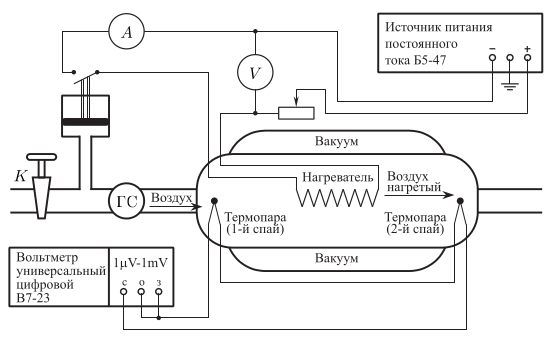
\includegraphics[width=1\linewidth]{images/installation.png}
        \begin{center}
            \caption{Схема установки}
        \end{center}
    \end{figure}
    Нагреватель в виде намотанной на пенопласт нихромовой проволоки расположен внутри калориметра непосредственно
     в воздушном потоке. Нагрев проволоки производится от регулируемого источника постоянного тока.
	Напряжение $U$ на нагревателе и ток $I$ через него регистрируются цифровыми мультиметрами. 
\subsection{Теоретический расчёт}
    Мощность нагрева равна $$N = UI \eqno{(3)} $$ Для измерения разности температур $\Delta T$ служит медно-константановая
	термопара. Один спай термопары расположен в струе воздуха, входящего в калориметр, и находится при комнатной 
    температуре, а второй — в струе выходящего нагретого воздуха. Константановая проволока термопары расположена
     внутри калориметра, а медные проводники подключены к цифровому вольтметру. Возникающая в термопаре ЭДС $\varepsilon$
      пропорциональна разности температур $\Delta T$ спаев: 
      $$ \varepsilon =\beta \Delta T, \eqno{(4)}$$ где $\beta = 40.7 \frac{\text{мкВ}}{^\circ C}$ — чувствительность 
      медно-константановой термопары в рабочем диапазоне температур (20–30 $^\circ C$ ). ЭДС регистрируется с 
      помощью микровольтметра.
	
	Объём воздуха, прошедшего через калориметр, измеряется газовым счётчиком ГС. Для регулировки расхода служит 
    кран К. Время $\Delta t$ прохождения некоторого объема $\Delta V$ воздуха измеряется секундомером. Объёмный 
    расход равен $\frac{\Delta V}{\Delta t} $, массовый расход может быть найден как 
    $$q = \rho_{0} \frac{\Delta V}{\Delta t}, \eqno{(5)} $$ где $rho_{0}$ — плотность воздуха при комнатной температуре,
     которая в свою очередь может быть получена из уравнения Менделеева–Клапейрона: 
     $\rho_{0}= \frac{\mu P_{0} }{R T_{0}},$ где $P_{0}$ — атмосферное давление, $T_{0}$ — комнатная температура
      (в Кельвинах), $\mu = 29,0 { \text{г}/\text{моль}}$ — средняя молярная масса (сухого) воздуха.

	Учитывая особенности устройства калориметра, следует ожидать, что мощность нагревателя расходуется
     не только на нагрев массы прокачиваемого воздуха, но и частично теряется за счет нагрева внутренних 
    стенок термостата и рассеяния тепла через торцы термостата. Можно предположить, что при небольшом 
    нагреве ($\Delta T \ll T_{0}$) мощность потерь тепла $N_{пот}$ прямо пропорциональна разности 
    температур:$$ N_{пот} = \alpha \Delta T, \eqno{(6)}$$ где $\alpha$ — некоторая константа. При этом 
    условии основное соотношение (2) принимает вид $$N = (c_{p}q +\alpha)\Delta T \eqno{(7)}$$ 
	Следовательно, при фиксированном расходе воздуха ($q = const$) подводимая мощность и разность температур
     связаны прямой пропорциональностью($\Delta T(N)$ — линейная функция).

\section{Результаты измерений и обработка данных}
\begin{enumerate}
    \item Подготовим к работе газовый счетчик: проверим, что он заполнен  водой, установим счетчик по уровню.
    \item Охладим калориметр до комнатной температуры.
    \item Включим вольтметр, предназначенный для измерения ЭДС термопары. 
    \item Запишем показания компнатной температуры и давления. $$T_{0} = 296.8 \pm 0.2 K $$ $$ P_{0} = 99260 \pm 20 \; {\text{Па}} $$
    \item Молярная масса воздуха $\mu = 28.97$ г/моль
    \item С помощью газового счетчика и секундомера измерим максимальный расход воздуха 
    $\frac{\Delta V}{\Delta T} \left[\frac{\text{л}}{\text{c}} \right]$. По найденным 
    значениям определим среднее значение расхода и массовый расход воздуха $q_{max} \left[\frac{\text{л}}{\text{c}} \right]$
    следующим образом: $$q = \rho_0 \frac{\Delta V}{\Delta t} = \frac{\mu P_0}{RT_0} \frac{\Delta V}{\Delta t}.$$
\end{enumerate}
    
    Относительная погрешность косвенных измерений может быть найдена по формуле: 
    $$\epsilon_{q_{max}} = \frac{\sigma_{q_{max}}}{q_{max}} = \sqrt{(\frac{\sigma_{T_0}}{T_{0}})^2 +
                                                                 (\frac{\sigma_{P_0}}{P_{0}})^2 +
                                                                 (\frac{\sigma_t}{t})^2} $$
\subsection{Эксперимент №1}
    В этом эксперименте устанавливаем расход $\approx 10 \frac{\text{л}}{\text{мин}}$
    Тогда $$q_1 = \frac{28.97 \cdot 10^{-3} \cdot 99260}{8.31 \cdot 296.8} \cdot 10 \cdot \frac{10^{-3}}{60}
     \approx 0.000194 \text{ кг/c} = 0.19 \text{ г/c}$$
     $$\mathcal{E}_{q_1} = \mathcal{E}_T + \mathcal{E}_{p_0} + \mathcal{E}_{\text{расход}} = 0.0007 + 0.002 + 0.006 \approx 0.01 = 1\%$$
    
    Приведем данные показаний приборов в \textbf{таблице 1}:
    \begin{table}[h]
        \centering
        \begin{tabular}{|c|c|c|c|c|c|} \hline
        № & $ U $, \text{В} & $ I $, \text{мА} & $ N $, \text{мВт} & $ \epsilon $, \text{мВ} & $ \Delta T $, K \\ \hline
        1 & 3.569 & 101.06 & 360.68  & 0.074 & 1.8 \\ \hline
        2 & 5.486 & 155.4  & 852.52  & 0.166 & 4.08 \\ \hline
        3 & 6.593 & 189.7  & 1250.69 & 0.255 & 6.26 \\ \hline
        4 & 7.599 & 215.9  & 1640.62 & 0.325 & 8.01 \\ \hline
        \shortstack{Среднее \\ значение} & & & 1026.13 & & 5.04 \\ \hline
        \end{tabular}
        \caption{$\Delta T(N)$ в 1ом эксперименте}
    \end{table}

\subsection{Эксперимент №2}
    В этом эксперименте устанавливаем расход $\approx 4.81 \frac{\text{л}}{\text{мин}}$
    Тогда $$q_2 = \frac{28.97 \cdot 10^{-3} \cdot 99260}{8.31 \cdot 296.8} \cdot 4.81 \cdot \frac{10^{-3}}{60}
     \approx 0.09 \text{ г/c}$$
    $$\mathcal{E}_{q_2} = \mathcal{E}_T + \mathcal{E}_{p_0} + \mathcal{E}_{\text{расход}} = 0.0007 + 0.002 + 0.006 \approx 0.01 = 1\%$$
    
    Приведем данные показаний приборов в \textbf{таблице 1}:
    \begin{table}[h]
        \centering
        \begin{tabular}{|c|c|c|c|c|c|} \hline
        № & $ U $, \text{В} & $ I $, \text{мА} & $ N $, \text{мВт} & $ \epsilon $, \text{мВ} & $ \Delta T $, K \\ \hline
        1 & 2.647 & 74.19  & 196.38 & 0.079 & 1.94 \\ \hline
        2 & 3.647 & 102.29 & 373.05 & 0.164 & 4.05 \\ \hline
        3 & 4.485 & 125.81 & 564.26 & 0.245 & 6.01 \\ \hline
        4 & 5.430 & 152.19 & 826.39 & 0.320 & 7.91 \\ \hline
        \shortstack{Среднее \\ значение} & & & 490.02 & & 4.98 \\ \hline
        \end{tabular}
        \caption{$\Delta T(N)$ во 2ом эксперименте}
    \end{table}

\subsection{Графики зависимости $N$ от $\Delta T$}
    Так как наша зависимлсть линейная, проходящая через точку $(0,0)$, то вычислить ее коэффициент наклона
    можно по методу наименьших квадратов $k = \frac{\langle \Delta T \cdot N \rangle}{\langle \Delta T^2 \rangle}$,
    а абсолютную погрешность можно посчитать следующим образом: $\sigma_k = \frac{1}{\sqrt{n}} \cdot 
    \sqrt{\frac{\langle \Delta N^2 \rangle}{\langle \Delta T^2 \rangle} - k^2}$ \\
    В первом случае: $k_1 = \frac{6271.35}{30.78} \approx 203.75 \text{ мВт/К}$ \\
    $\sigma_{k_1} = \frac{1}{\sqrt{4}} \cdot \sqrt{\frac{1278185}{30.78} - 203.75^2} \approx 1.76 \text{ мВт/К}$ \\
    Во втором случае: $k_2 = \frac{2954.93}{29.71} \approx 99.46 \text{ мВт/К}$
    $\sigma_{k_2} = \frac{1}{\sqrt{4}} \cdot \sqrt{\frac{294760}{29.71} - 99.46^2} \approx 2.69 \text{ мВт/К}$ \\
    \begin{figure}[H]
        \centering
        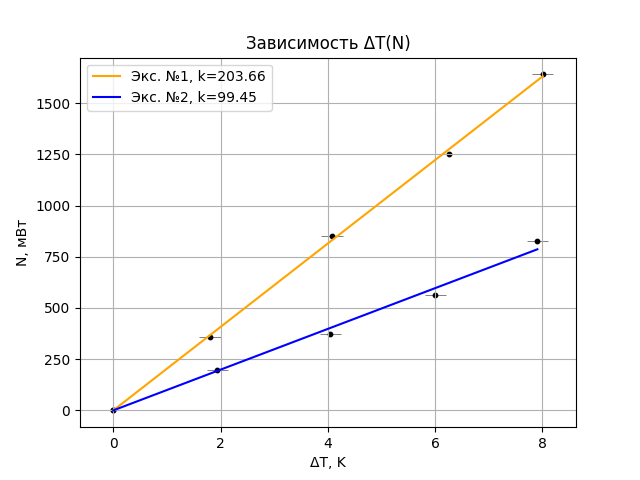
\includegraphics[width=1\linewidth]{graphs/figure1.png}
        \begin{center}
            \caption{График зависимости $N$ от $\Delta T$}
        \end{center}
    \end{figure}
    Из ситсемы уравнений 
    $$\begin{cases}
        c_{p}q_1 +\alpha = k_1 \\
        c_{p}q_2 +\alpha = k_2
    \end{cases}$$
    получаем, что $c_p = \frac{k_1 - k_2}{q_1 - q_2} = \frac{(203.75 - 99.46) \cdot 60 \cdot 10^{-3}}{(10 - 4.81) \cdot 10^{-3}}
     \approx 1205.7 \text{ Дж/(кг$\cdot$К)}$ \\
    При этом $\mathcal{E}_{c_p} = max\{\mathcal{E}_{k_1}; \mathcal{E}_{k_2}\} + max\{\mathcal{E}_{q_1}; \mathcal{E}_{q_2}\}
     = \mathcal{E}_{k_2} + \mathcal{E}_{q_2} = \frac{\delta_{k_2}}{k_2} + \frac{\delta_{q_2}}{q_2} =
     \frac{2.69}{99.46} + 0.01 = 0.037 \approx 3.7\%$ \\
    Тогда $\alpha = k_1 - c_{p}q_1 = \frac{q_1 \cdot k_2 - q_2 \cdot k_1}{q_1 - q_2} =
     \frac{(10 \cdot 99.46 - 4.81 \cdot 203.75) \cdot 10^{-3}}{10-4.81} = 2.8 \text{ мВт/c}$ \\
    Аналогично $c_p$ можно получить $\mathcal{E}_\alpha \approx 4\%$
\section{Обсуждение результатов}
    В результате работы мы:
    \begin{itemize}
        \item Нашли теплоемкость воздуха при нормальных условиях и определили коэффициент теплопотерь.
    
        \item Получили зависимость $N(\Delta T)$. Как нетрудно убедиться по рис. 2,
        во всех случаях аппроксимация прямой действительно применима, причем с очень
        хорошей точностью.

        \item Получили следующиую теплоемкость и коэффициент теплопотерь соответственно:
        $$c_p = (1205 \pm 45)\frac{\text{Дж}}{\text{кг} \cdot K}$$
        $$\alpha = (2.8 \pm 0.1)\frac{\text{Дж}}{K}$$
    \end{itemize}
\end{document}
